\clearpage
\begin{proofbox}
\textbf{方法一：最快证明（考场三步速写）}

\begin{center}
% C093: a=4, A=1, c=2; E: x^2/16+y^2/12=1, H: x^2-y^2/3=1
% Intersection P=(2,3); PF1=5, PF2=3; generated as exact coordinate constructions.
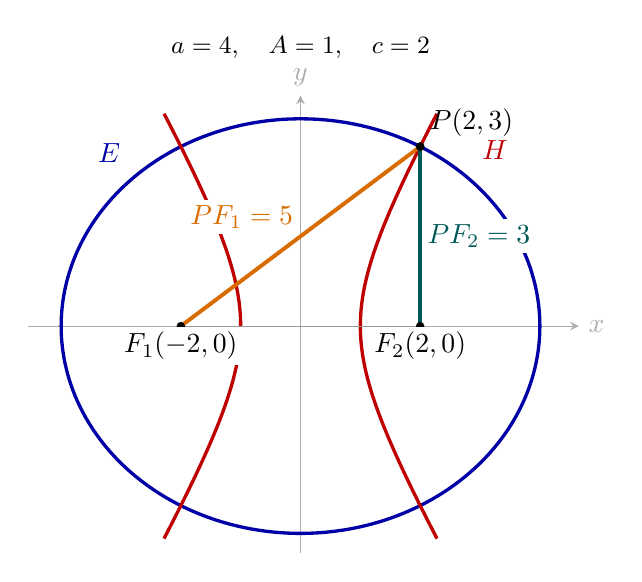
\begin{tikzpicture}[scale=0.76,>=stealth]
 \node[font=\small] at (0,4.65) {$a=4,\quad A=1,\quad c=2$};
 \draw[->,gray!65] (-4.55,0)--(4.65,0) node[right]{$x$};
 \draw[->,gray!65] (0,-3.8)--(0,3.85) node[above]{$y$};
 \draw[blue!65!black,very thick,samples=160,domain=0:360,smooth,variable=\t]
  plot ({4*cos(\t)},{sqrt(12)*sin(\t)});
 \draw[red!75!black,very thick,samples=110,domain=-3.55:3.55,variable=\t]
  plot ({sqrt(1+\t*\t/3)},{\t});
 \draw[red!75!black,very thick,samples=110,domain=-3.55:3.55,variable=\t]
  plot ({-sqrt(1+\t*\t/3)},{\t});
 \coordinate (L) at (-2,0); \coordinate (R) at (2,0); \coordinate (P) at (2,3);
 \draw[orange!85!black,line width=1.4pt] (L)--(P) node[midway,above left,fill=white,inner sep=2pt]{$PF_1=5$};
 \draw[teal!70!black,line width=1.4pt] (R)--(P) node[midway,right,fill=white,inner sep=2pt]{$PF_2=3$};
 \draw[gray!80] (L)--(R);
 \fill (L) circle (2pt) node[below,fill=white,inner sep=2pt]{$F_1(-2,0)$};
 \fill (R) circle (2pt) node[below,fill=white,inner sep=2pt]{$F_2(2,0)$};
 \fill (P) circle (2.1pt) node[above right]{$P(2,3)$};
 \node[blue!65!black] at (-3.2,2.9) {$E$};
 \node[red!75!black] at (3.25,2.95) {$H$};
\end{tikzpicture}

\end{center}
图中同一个 $P$ 同时在蓝色椭圆与红色双曲线上，
两条彩色焦半径同时受“定和”与“定差”约束。

\textbf{第1步，写定义：}设 $r_1=PF_1,r_2=PF_2$，由同一个公共点满足两条曲线的定义，
\[r_1+r_2=2a,\qquad |r_1-r_2|=2A.\]
\textbf{第2步，解和差：}较长、较短焦半径分别为
\[
\frac{(2a)+(2A)}2=a+A,\qquad
\frac{(2a)-(2A)}2=a-A.
\]
\textbf{第3步，判支别：}右支距离左焦点更远，左支距离右焦点更远，所以
\[
\boxed{\begin{array}{ll}
x_P>0:&r_1=a+A,\quad r_2=a-A,\\[2pt]
x_P<0:&r_1=a-A,\quad r_2=a+A.
\end{array}}
\]
\textbf{识别信号：}一看到“共焦＋公共点”求焦半径，先写定义，
不必先联立两条标准方程。
\end{proofbox}

\clearpage
\begin{proofbox}
\textbf{方法二：最低门槛证明（平均值＋一半差）}

\begin{center}
% C093：长度分解教学图；真实线段长度与 9:7:5:2 一致。
% 长焦半径=9=7+2，短焦半径=5=7-2。
\begin{tikzpicture}[x=0.76cm,y=0.88cm,>=stealth]
  % 平均值分界 7
  \draw[gray!65,densely dashed] (7,-0.9)--(7,2.65);
  \node[gray!70!black,above] at (7,2.65) {$a=7$};
  \node[anchor=west] at (-0.4,3.2) {\textbf{同一平均值 $7$，一长一短}};
  % Long bar 0..7 plus 7..9
  \draw[teal!70!black,line width=5pt] (0,1.9)--(7,1.9);
  \draw[orange!88!black,line width=5pt] (7,1.9)--(9,1.9);
  \draw[black,thin] (0,1.62)--(0,2.18) (9,1.62)--(9,2.18);
  \node[anchor=east] at (-0.3,1.9) {较长};
  \node[above,teal!70!black] at (3.4,1.97) {$a=7$};
  \node[above,orange!88!black] at (8.0,1.97) {$A=2$};
  \node[anchor=west] at (9.3,1.9) {$9=7+2$};
  % Short bar 0..5, dashed deficit to avg length=7
  \draw[teal!70!black,line width=5pt] (0,0.15)--(5,0.15);
  \draw[orange!85!black,densely dashed,line width=1.7pt] (5,0.15)--(7,0.15);
  \draw[black,thin] (0,-0.12)--(0,0.43) (5,-0.12)--(5,0.43);
  \node[anchor=east] at (-0.3,0.15) {较短};
  \node[above,teal!70!black] at (2.4,0.22) {$a-A=5$};
  \node[below,orange!88!black] at (6,-0.05) {少 $2$};
  \node[anchor=west] at (9.3,0.15) {$5=7-2$};
  \node[gray!75!black,anchor=west] at (0,-1.5) {实线是真实长度，虚线表示“距平均值还差 $2$”。};
\end{tikzpicture}

\end{center}

\textbf{第一步：}椭圆规定两条焦半径总长 $2a$，
所以每条长度的\emph{平均值}是 $a$。

\textbf{第二步：}双曲线规定两条长度相差 $2A$，
一条比平均值多 $A$，另一条比平均值少 $A$。
因此不论公共点在哪里，长短两条的长度都是
\[\boxed{a+A\quad\text{和}\quad a-A}.\]

\textbf{第三步：}右支点离左焦点远，把长的分配给 $PF_1$；
左支点离右焦点远，把长的分配给 $PF_2$。
也可由
\[PF_1^2-PF_2^2=4cx_P\]
检验远近。$a>c>A>0$ 保证短的一条也严格大于 $0$。

\textbf{这套方法的价值：}即使一时忘记代数加减消元，
仍可用“平均数与偏离量”重新想出公式。
\end{proofbox}

\clearpage
\begin{proofbox}
\textbf{方法三：常规坐标法（联立标准方程＋距离公式）}

\begin{center}
% Exact representative: c=3, a=5, A=2,
% P=(10/3,4sqrt(5)/3), PF1=7, PF2=3.
% Both right triangles share PQ; horizontal legs are x_P+c and x_P-c.
\begin{tikzpicture}[x=0.95cm,y=0.95cm,>=stealth,font=\small]
 \coordinate (L) at (-3,0);
 \coordinate (R) at (3,0);
 \coordinate (P) at ({10/3},{4*sqrt(5)/3});
 \coordinate (Q) at ({10/3},0);
 \draw[->,gray!65] (-3.9,0)--(4.55,0) node[right]{$x$};
 \draw[->,gray!65] (0,-0.35)--(0,3.85) node[above]{$y$};
 \draw[orange!85!black,very thick] (L)--(P)
   node[pos=0.46,above left,fill=white,inner sep=2pt]{$r_1=PF_1$};
 \draw[teal!70!black,very thick] (R)--(P)
   node[pos=0.55,right=5pt]{$r_2=PF_2$};
 \draw[densely dashed,gray!80] (P)--(Q);
 \draw[gray!80] ({10/3-0.17},0)--({10/3-0.17},0.17)--({10/3},0.17);
 \node[anchor=west] at (3.7,3.42) {$P(x_P,y_P)$};
 \node[anchor=east,fill=white,inner sep=2pt] at (2.72,1.02) {$PQ=|y_P|$};
 \draw[gray!70] (2.77,1.02)--({10/3},1.02);
 \fill (L) circle (2pt) node[below=4pt]{$F_1(-c,0)$};
 \fill (R) circle (2pt) node[below left=4pt]{$F_2(c,0)$};
 \fill (P) circle (2pt);
 \fill (Q) circle (1.6pt) node[below right=4pt]{$Q(x_P,0)$};
 \draw[<->,orange!85!black] (-3,-0.95)--({10/3},-0.95)
   node[midway,below]{$F_1Q=x_P+c$};
 \node[teal!70!black,anchor=west] at (0.4,-2.05) {$F_2Q=x_P-c$（此图 $x_P>c$）};
 \draw[teal!70!black] ({19/6},-0.1)--(4.3,-1.65)--(4.3,-1.82);
 \node[anchor=west] at (-3.6,4.55) {\textbf{两条距离共用同一高度 $PQ$}};
 \node[anchor=west] at (-3.6,-2.85) {一般情形水平距离取绝对值，平方后仍为 $(x_P\pm c)^2$。};
\end{tikzpicture}

\end{center}
过 $P$ 向 $x$ 轴作垂线，垂足为 $Q$。图中两个直角三角形
共用高度 $|y_P|$，分别给出距离平方 $(x_P+c)^2+y_P^2$、
$(x_P-c)^2+y_P^2$；一般位置的水平距离应取绝对值。

\end{proofbox}
\clearpage
\begin{proofbox}
\textbf{方法三（续）：先求坐标平方，再还原正长度。}

\textbf{第1步：}由共焦条件，写出同一个公共点的两条方程：
\[
\boxed{\frac{x^2}{a^2}+\frac{y^2}{b^2}=1},\qquad
\boxed{\frac{x^2}{A^2}-\frac{y^2}{B^2}=1},
\]
其中 $a>b>0$、$A,B>0$，且
\[\boxed{a^2-b^2=A^2+B^2=c^2}.\]
两式分别整理为
\[
 y^2=b^2\left(1-\frac{x^2}{a^2}\right),\qquad
 y^2=B^2\left(\frac{x^2}{A^2}-1\right).
\]
\textbf{第2步：}同一个公共点的纵坐标平方 $y^2$ 相同，
因此让两式相等，消去 $y^2$：
\[
 b^2+B^2=x^2\left(\frac{b^2}{a^2}+\frac{B^2}{A^2}\right).
\]
用共焦条件 $b^2=a^2-c^2$、$B^2=c^2-A^2$ 代入：
\[
 a^2-A^2
 =c^2x^2\left(\frac1{A^2}-\frac1{a^2}\right)
 =\frac{c^2x^2(a^2-A^2)}{a^2A^2}.
\]
因为 $a>c>A>0$，所以 $a^2-A^2>0$，可以约去，得到
\[
\boxed{x^2=\frac{a^2A^2}{c^2}}.
\]
将其代入椭圆方程，再利用 $c^2-A^2=B^2$，得到
\[
y^2=b^2\left(1-\frac{A^2}{c^2}\right)
=\boxed{\frac{b^2B^2}{c^2}}>0.
\]
\textbf{第3步：}由距离公式和已求得的 $x^2,y^2$，
\[
\begin{aligned}
PF_1^2&=(x+c)^2+y^2=a^2+A^2+2cx,\\
PF_2^2&=(x-c)^2+y^2=a^2+A^2-2cx.
\end{aligned}
\]
当 $x=aA/c>0$ 时，两式为
$(a+A)^2$、$(a-A)^2$；当 $x<0$ 时交换。
因为焦半径是正长度，取正平方根就得到主结论。

\textbf{方法定位：}坐标法较慢，但适合题目还要求验证公共点位置时使用；
若主要目标是求四个公共点的坐标，转入 C094。
\end{proofbox}

\clearpage
\begin{proofbox}
\textbf{补充：两点距离平方相减，快速检查左右支。}

\begin{center}
% Exact representative: c=3, a=5, A=2,
% P=(10/3,4sqrt(5)/3), PF1=7, PF2=3.
% Both right triangles share PQ; horizontal legs are x_P+c and x_P-c.
\begin{tikzpicture}[x=0.95cm,y=0.95cm,>=stealth,font=\small]
 \coordinate (L) at (-3,0);
 \coordinate (R) at (3,0);
 \coordinate (P) at ({10/3},{4*sqrt(5)/3});
 \coordinate (Q) at ({10/3},0);
 \draw[->,gray!65] (-3.9,0)--(4.55,0) node[right]{$x$};
 \draw[->,gray!65] (0,-0.35)--(0,3.85) node[above]{$y$};
 \draw[orange!85!black,very thick] (L)--(P)
   node[pos=0.46,above left,fill=white,inner sep=2pt]{$r_1=PF_1$};
 \draw[teal!70!black,very thick] (R)--(P)
   node[pos=0.55,right=5pt]{$r_2=PF_2$};
 \draw[densely dashed,gray!80] (P)--(Q);
 \draw[gray!80] ({10/3-0.17},0)--({10/3-0.17},0.17)--({10/3},0.17);
 \node[anchor=west] at (3.7,3.42) {$P(x_P,y_P)$};
 \node[anchor=east,fill=white,inner sep=2pt] at (2.72,1.02) {$PQ=|y_P|$};
 \draw[gray!70] (2.77,1.02)--({10/3},1.02);
 \fill (L) circle (2pt) node[below=4pt]{$F_1(-c,0)$};
 \fill (R) circle (2pt) node[below left=4pt]{$F_2(c,0)$};
 \fill (P) circle (2pt);
 \fill (Q) circle (1.6pt) node[below right=4pt]{$Q(x_P,0)$};
 \draw[<->,orange!85!black] (-3,-0.95)--({10/3},-0.95)
   node[midway,below]{$F_1Q=x_P+c$};
 \node[teal!70!black,anchor=west] at (0.4,-2.05) {$F_2Q=x_P-c$（此图 $x_P>c$）};
 \draw[teal!70!black] ({19/6},-0.1)--(4.3,-1.65)--(4.3,-1.82);
 \node[anchor=west] at (-3.6,4.55) {\textbf{两条距离共用同一高度 $PQ$}};
 \node[anchor=west] at (-3.6,-2.85) {一般情形水平距离取绝对值，平方后仍为 $(x_P\pm c)^2$。};
\end{tikzpicture}

\end{center}
观察共用的垂线 $PQ$：两条距离平方相减时，高度平方 $y_P^2$ 抵消。

把 $PF_1$ 和 $PF_2$ 平方相减，
\[
PF_1^2-PF_2^2=4cx_P
=(PF_1-PF_2)(PF_1+PF_2).
\]
右支 $x_P>0$，故左边大于零，$PF_1-PF_2=2A$；
左支 $x_P<0$，故左边小于零，$PF_1-PF_2=-2A$。
利用 $PF_1+PF_2=2a$，两个支别的公式便得到独立核查。

\textbf{关键意义：}相减不是机械消元；它让两次出现的 $y_P^2$
消失，直接读出点在左侧还是右侧。若只为求焦半径，
无需进一步求交点坐标。
\end{proofbox}
